\cotefile{71}
\scanpage{11}
% archive sheet number: 10
% The calculation on the left half turns through 180 degrees.
\[
\begin{aligned}
t^2(\lambda_0)&=\lambda_0\\
t^2(\lambda_1)&=t(g_{\unsure{v|\nu}})\underbrace{t(\lambda_v)}_{\lambda_1}t(g_v)^{-1}
\end{aligned}
\]

\[
\lambda_0\quad\lambda_1\quad\lambda_2
\qquad\qquad \text{\uline{$t^2=\mathrm{int}$}}(\lambda_0)
\]
\[
\begin{aligned}
t(\lambda_0)&=\lambda_0\\
t(\lambda_1)&=\lambda_1\lambda_2\lambda_1^{-1}=\lambda_0^{-1}\lambda_2\lambda_0\\
t(\lambda_2)&=\lambda_1
\end{aligned}
\]

\[
\begin{aligned}
t^2(\lambda_0)&=\lambda_0\\
t^2(\lambda_1)&=(\lambda_1\lambda_2\deleted{\lambda_1^{-1}})\deleted{\lambda_1}
   (\lambda_1\lambda_2^{-1}\lambda_1^{-1})\\
 &=\lambda_1\underbrace{\lambda_2\lambda_1\lambda_2^{-1}}\lambda_1^{-1}\\
 &=\mathrm{int}(\lambda_1\unsure{,|\cdot}\lambda_2)\lambda_1
   =\mathrm{int}(\lambda_0^{-1})\lambda_1\\
t^2(\lambda_2)&=t(\lambda_1)=\lambda_1\lambda_2\lambda_1^{-1}
   =\deleted{\unsure{\mathrm{int}(\lambda_1|\mathrm{id}(\lambda_1}}\unsure{)}\\
 &=(\lambda_1\lambda_2)\lambda_2(\lambda_2^{-1}\lambda_1^{-1})\\
 &=\mathrm{int}(\lambda_{\unsure{1|0}}\lambda_2)\lambda_2\,\unsure{\mathrm{int}(\lambda_1|\mathrm{id}(\lambda_1}
\end{aligned}
\]
% Detached short pen stroke beside the last line on the rotated half.
\margin{$\unsure{\cdot|\prime}$}

% Upright half of the sheet.
\diagram{\begin{tikzcd}[ampersand replacement=\&,column sep=large]
\deleted{\unsure{A|H}}\,G/H
 \& \unsure{\widetilde E|E}=\unsure{G|\mathbb G}\unsure{\wedge|\times}_{H}\unsure{E|\mathbb E} \arrow[l]\arrow[d]
 \& G\times_{H}E\arrow[l]\arrow[d]\\
 e\arrow[u,no head]\arrow[r,no head]
 \& E\arrow[ul] \& E'\arrow[l]
\end{tikzcd}}

\diagram{\begin{tikzcd}[ampersand replacement=\&,column sep=small,row sep=large]
 B_H \arrow[d,"f"',no head] \& E_H
 \& \vphantom{E}\arrow[d,no head,start anchor=north,end anchor=south] \& \unsure{f_!|h_!} f^{*}(E)\arrow[r] \& E\arrow[l,bend right=20,dashed]\\
 B_G\unsure{-|{}} \& E^{\unsure{'|{}}} \& \vphantom{E}
 \& f^{*}f_!(f^{\unsure{*|H}}E)\arrow[r]
 \& f^{*}E\arrow[l,bend left=20]
\end{tikzcd}}

\[
\widetilde E\simeq
\]
\scanpage{12}
% archive sheet number: 11
3) Supposons $\dot K\cap C=\emptyset$, et posons
\[
\begin{aligned}
 \unsure{\cdot|{}}B'&=U'_K\cap\dot K\\
 U'&=U'_K\setminus B'=\mathrm{Int}\unsure{(|{}}U'_K)\\
 V'&=X\setminus\overline{U'_K}=(\underbrace{X\setminus U'_K}_{X'_1})\setminus C\\
   &=\mathrm{Int}(X'_1)
\end{aligned}
\]
\[
\deleted{\unsure{U'=U'_K|U=U_K}}
\]
enfin $W=V\cap V'=\complement K$.

\diagram{\begin{tikzcd}[ampersand replacement=\&,row sep=large,column sep=small]
 U^{\deleted{\unsure{'|1}}}\arrow[dr,no head,"B"'] \& \& U'\arrow[ll,"C"']\arrow[dl,no head,"B'"']\\
 \unsure{\cdot|{}} \& W^{\deleted{\unsure{U|V}}} \&
\end{tikzcd}}

\figure{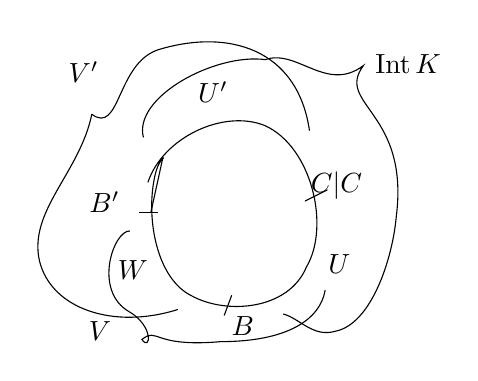
\begin{tikzpicture}[x=0.95cm,y=0.95cm]
\draw (0.88,3.06) .. controls (1.26,2.78) and (1.21,3.73) .. (1.76,3.92)
 .. controls (2.7,4.21) and (3.63,3.94) .. (3.79,2.84);
\draw (0.88,3.06) .. controls (0.72,2.28) and (0.03,1.77) .. (0.18,1.1)
 .. controls (0.34,0.45) and (1.18,0.18) .. (2.03,0.45);
\draw (1.57,2.75) .. controls (1.43,3.29) and (2.53,3.88) .. (3.20,3.79)
 .. controls (3.62,3.94) and (4.02,3.34) .. (4.51,3.71)
 .. controls (4.13,3.19) and (5.13,3.10) .. (4.95,1.69)
 .. controls (4.9,1.13) and (4.62,0.26) .. (4.14,0.16)
 .. controls (3.84,0.07) and (3.66,0.33) .. (3.44,0.39);
\draw (1.39,1.5) .. controls (1.17,1.51) and (0.89,0.70) .. (1.38,0.42)
 .. controls (1.72,0.22) and (1.66,-0.12) .. (1.55,0.05)
 .. controls (1.77,0.22) and (1.68,-0.06) .. (2.60,0.02)
 .. controls (3.47,0.02) and (3.93,0.30) .. (4.00,0.71);
\draw (1.63,2.15) .. controls (1.83,2.75) and (2.64,3.13) .. (3.19,2.91)
 .. controls (3.82,2.63) and (4.07,1.56) .. (3.75,1.02)
 .. controls (3.51,0.44) and (2.68,0.38) .. (2.22,0.63)
 .. controls (1.76,0.85) and (1.61,1.62) .. (1.71,2.17)
 .. controls (1.74,2.34) and (1.78,2.42) .. (1.84,2.48);
\draw (1.83,2.48)--(1.67,1.75);
\draw (1.51,1.75)--(1.76,1.75);
\draw (3.73,1.90)--(4.03,2.05);
\draw (2.75,0.64)--(2.65,0.37);
\node at (0.77,3.62) {$V'$}; \node at (2.50,3.36) {$U'$};
\node[right] at (4.54,3.73) {$\mathrm{Int}\,K$};
\node at (1.05,1.89) {$B'$}; \node at (4.15,2.11) {$\unsure{C|\mathbb C}$};
\node at (1.43,0.98) {$W$}; \node at (4.19,1.06) {$U$};
\node at (0.99,0.16) {$V$}; \node at (2.90,0.23) {$B$};
\end{tikzpicture}}

Alors on a :
\[
\begin{array}{ll|l}
 U,U',W&\text{ouverts disjoints}& U,U',W,B,B',C\\
 B,B',C&\text{fermés disjoints}&\text{pseudopartition de }X
\end{array}
\]
\[
\left\{\begin{aligned}
 &\overline U\cap\overline{U'}=C,\quad
 \overline U^{\deleted{\unsure{'|*}}}\cap\overline W=B,\quad
 \overline W\cap\overline{U'}=B'\\
 &\unsure{\dot U'|\overline{U'}}\deleted{\unsure{\setminus|{}}}=\overline{U'}\setminus U'=B'\cup C,\quad
 \dot U=B\cup C,\quad \dot W=B\cup B'\\
 &K=\overline{U\cup U'}=\complement W=(U\cup U')\cup B\cup B'\cup C,\quad
 \mathrm{Int}\,K=\unsure{(|{}}U\cup U'\cup C
\end{aligned}\right.
\]
\deleted{\illegible{1}}

4) \deleted{\unsure{Donnons|Donnés}} Soient $U,U',W$ 3 ouverts d'un espace $X$.

Conditions équivalentes

a) $U,U',W$ \unsure{mutuellement} disjoints, réunion dense,
\[
 \overline U\cap\overline{U'}\cap\overline W=\emptyset,\quad
 \deleted{\unsure{\overline U|U}}\dot U\subset\overline{U'\cup W},\quad
 \dot U'\subset\overline{U\deleted{\unsure{\cap|'}}\cup W},\quad
 \dot W\subset\overline{U\cup U'}
\]

b) \unsure{Posant} $C=\overline U\cap\overline{U'}$, $B=\overline U\cap\overline W$, $B'=\overline W\cap\overline{U'}$, les 6 ens $U,U',W,B,B',C$ forment une pseudopartition de $X$.

On a alors les relations ci-dessus \unsure{--|$\cdots$}

Il revient au \unsure{$=$} de se donner (pour $X$ \unsure{fixé}) $U,U',W$ satisfaisant les conditions \inserted{équ.} a) b), ou $K,$ \inserted{fermé de $X$} et $\underbrace{U_K,U'_K}_{\text{ouverts de }K}$ satisfaisant
\[
\left\{\begin{aligned}
 \overline{U_K}&=K\setminus U'_K,\quad \overline{\unsure{W_K|U'_K}}=K\setminus U_K\\
 C\cap\dot K&=\emptyset\quad \text{\unsure{où}}\quad C=\overline{U_K}\cap\overline{U'_K}=K\setminus(U_K\cup U'_K)
\end{aligned}\right.
\]
\scanpage{13}
% archive sheet number: 12
% A fine diagonal stroke crosses the writing from the upper D(d) down
% to the last group. The last group is also crossed by short diagonals.
\diagram{\deleted{\mbox{\begin{tikzcd}[ampersand replacement=\&,column sep=small,row sep=large,font=\footnotesize]
d \& D(d)=\pi_0\Sigma_d(\unsure{\mathfrak X|\mathscr X|\mathcal X|X})
 \arrow[r,"{\overset{\alpha_d}{\sim}}"]\arrow[d,"{R_{d',d}}"]
 \& E(d)\overset{\text{dfn}}{=}\{e\in E\mid\varphi(M(e))=d\}
 \arrow[d,"{r_{d',d}}"]\\
 \shortstack{$\cup$\\$d'$} \& D(d')\arrow[r,"{\overset{\alpha_{d'}}{\sim}}"]
 \& E(d')
\end{tikzcd}}}}

\diagram{\deleted{\mbox{\begin{tikzcd}[ampersand replacement=\&,column sep=small,row sep=small,font=\footnotesize]
D(\{i\})=\pi_0\unsure{[|{}}\deleted{\unsure{\Delta|X}}\Sigma(X_i,\partial X_i)
 \arrow[r,"{\overset{\alpha_i}{\sim}}"]
 \& E(\{i\})=\varphi^{-1}(\{i\})\\
 \begin{array}{cc}\Vert&\backslash\\[-2pt]
 \displaystyle\bigcup_{\unsure{\mu|p}\varphi(M(e))\le i}|E_e|,
 &\displaystyle\bigcup_{\mu\varphi\unsure{(|\lvert}M(e)<i}\unsure{(|\lvert}E_e\rvert
 \end{array} \&
\end{tikzcd}}}}

\[
\deleted{\partial X_i=\bigcup_{\mu(\varphi(M(e)))<i}|E_e|}
\]
\[
\deleted{\partial X_i\overset{\text{dfn}}{=}\bigcup_{j<i}X_j
 =\bigcup_{j<i}\ \bigcup_{\substack{e\in E\\\varphi M\unsure{(|{}}e)\le j}}|E_e|
 =\bigcup_{\substack{e\in E\\\exists\,j\ \text{tel que}\\\varphi\unsure{\mathord{.}|{}}(M\unsure{\mathord{.}|{}}(e))\le j<i}}|E_e|}
\]
\figure{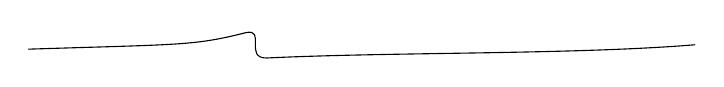
\begin{tikzpicture}[x=0.7cm,y=0.7cm]
\draw (0,0) .. controls (2.8,0.09) and (3.0,0.06) .. (3.95,0.30)
 .. controls (4.32,0.38) and (3.91,-0.17) .. (4.33,-0.16)
 .. controls (6.6,-0.05) and (9.9,-0.10) .. (12.1,0.08);
\end{tikzpicture}}

\[
\deleted{|\unsure{\mathcal K|K|k}|=(K_0,K)\supset(L_0,L)=|L|}
\qquad\unsure{\mathrel{.\mkern2mu:}}
\]
\diagram{\deleted{\mbox{\begin{tikzcd}[ampersand replacement=\&,row sep=tiny,column sep=0pt]
 \& \deleted{\unsure{\alpha|x}}\arrow[d,bend left=14] \&\\
 \&\deleted{\unsure{X|K}}\&\\
 \Sigma \& ( \& |K|,|L|)=|\Delta|
\end{tikzcd}}}}
\[
\deleted{\widetilde{\deleted{K}\unsure{\Delta|K}}\overset{\text{dfn}}{=}
 \Sigma(K,L)=(\widetilde{\deleted{K}\Delta}_0,\widetilde{\deleted{K}\Delta})}
\]
\[
\deleted{\left\{\begin{aligned}
 \widetilde{\deleted{K}\Delta}_0&=\varinjlim_{\sigma\in K\setminus L}
 \underset{\unsure{\cdot|{}}}{\sigma}\;(\subset{\deleted{\Delta}K}_0)\xrightarrow{\pi}{\deleted{\Delta}K}_0\\
 \widetilde{\deleted{K}\Delta}&=\mathrm{Im}\bigl((K\setminus L)\longrightarrow
 \unsure{\mathcal P|P}(\Delta_0)\bigr)
\end{aligned}\right.}
\]

\diagram{\deleted{\mbox{\begin{tikzcd}[ampersand replacement=\&,row sep=small,column sep=small]
 \deleted{\unsure{\Sigma|E}}|\widetilde{\deleted{K}\Delta}|\arrow[r,"?"]
 \& \Sigma(|K|,|L|)\\
 \Vert \& \sigma'=\mathrm{Im}(\sigma) \& \underline{\sigma}\in K\setminus L\\
 \displaystyle\varinjlim_{\sigma'\in\Delta}|\sigma'| \&
 |\sigma|\arrow[r]\arrow[rr,bend right=12] \& |\sigma'|\arrow[r] \& \Sigma
\end{tikzcd}}}}
\scanpage{14}
% archive sheet number: 13
\[
\begin{aligned}
 \Gamma_1&\unsure{:|=}\Gamma'_2\cup\Gamma'_3\\
 \Gamma_2&=\Gamma'_3\cup\Gamma'_1\\
 \Gamma_3&:\Gamma'_1\cup\Gamma'_2
\end{aligned}
\]

\diagram{\begin{tikzcd}[ampersand replacement=\&,column sep=small,row sep=small,font=\small]
 \& {\begin{gathered}\mathrm{a)}\quad\unsure{v|\nu}_1,v_2,v_3\\
 \text{\deleted{appartiennent}\inserted{\unsure{contenus}} dans}\\
 \text{régions distinctes}\\[-2pt]\text{de }E-\Gamma\end{gathered}}
 \arrow[d,Rightarrow] \\
 {\begin{gathered}\mathrm{a}')\ E-\Gamma\text{ a}\\
 \text{trois régions}\\\text{distinctes}\end{gathered}}\arrow[ur,Leftrightarrow]
 \& {\begin{gathered}\mathrm{b)}\quad\Gamma_1,\Gamma_2,\Gamma_3\text{ sont des courbes de}\\
 \text{Jordan}\end{gathered}}\arrow[d,Rightarrow]\\
 \&{\begin{gathered}\mathrm{c)}\quad\Gamma_1,\Gamma_2\text{ sont des courbes}\\
 \text{de Jordan}\end{gathered}}
\end{tikzcd}}

\figure{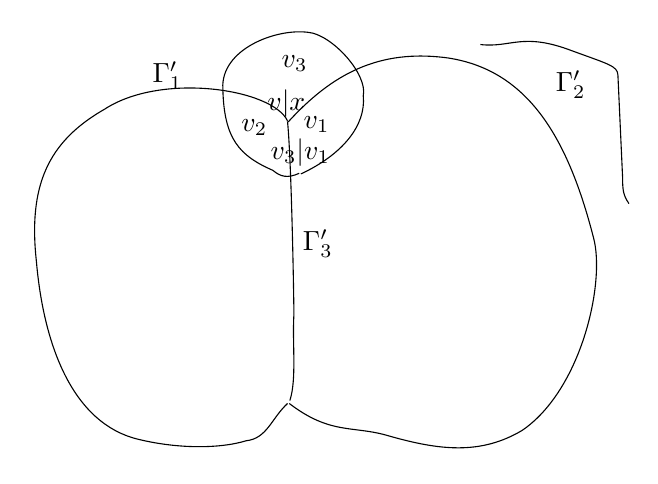
\begin{tikzpicture}[x=0.74cm,y=0.74cm]
\draw (4.34,5.59) .. controls (4.08,6.14) and (2.18,6.43) .. (1.20,5.79)
 .. controls (0.22,5.23) and (-0.11,4.47) .. (0.03,3.18)
 .. controls (0.16,1.68) and (0.68,0.40) .. (1.76,0.13)
 .. controls (2.44,-0.04) and (3.17,-0.04) .. (3.63,0.10)
 .. controls (3.99,0.14) and (4.06,0.48) .. (4.34,0.74);
\draw (4.35,5.57) .. controls (5.10,6.39) and (5.90,6.83) .. (7.09,6.67)
 .. controls (8.49,6.46) and (9.16,5.26) .. (9.59,3.59)
 .. controls (9.80,2.83) and (9.39,0.98) .. (8.37,0.28)
 .. controls (7.65,-0.15) and (6.94,-0.06) .. (6.09,0.18)
 .. controls (5.47,0.37) and (5.09,0.19) .. (4.37,0.74);
\draw (4.34,5.58) .. controls (4.40,4.97) and (4.44,3.09) .. (4.45,2.28)
 .. controls (4.42,1.76) and (4.50,1.16) .. (4.38,0.79);
\draw (4.57,4.68) .. controls (5.28,5.01) and (5.69,5.51) .. (5.64,6.02)
 .. controls (5.72,6.40) and (5.09,7.08) .. (4.69,7.11)
 .. controls (4.14,7.18) and (3.19,6.82) .. (3.23,6.14)
 .. controls (3.25,5.27) and (3.52,4.99) .. (4.09,4.74)
 .. controls (4.22,4.63) and (4.34,4.60) .. (4.54,4.69);
\draw (7.65,6.90) .. controls (8.18,6.84) and (8.37,7.12) .. (9.23,6.79)
 .. controls (9.86,6.56) and (10.00,6.53) .. (10.01,6.38)
 --(10.09,4.63) .. controls (10.09,4.41) and (10.10,4.31) .. (10.20,4.17);
\node at (2.28,6.36) {$\Gamma'_1$};
\node at (9.20,6.21) {$\Gamma'_2$}; \node at (4.86,3.48) {$\Gamma'_3$};
\node at (4.46,6.58) {$v_3$}; \node at (3.77,5.47) {$v_2$};
\node at (4.84,5.52) {$v_1$}; \node at (4.32,5.88) {$\deleted{\unsure{v|x}}$};
\node at (4.56,5.05) {$\deleted{\unsure{v_3|v_1}}$};
\end{tikzpicture}}

\[
\begin{aligned}
 &\mathrm{a)}\longleftrightarrow\mathrm{a}')\\
 &\mathrm{b)}\Longrightarrow\mathrm{c)}\deleted{\unsure{\Rightarrow|\Leftrightarrow}}\ \text{\unsure{triv.}}\\
 &\unsure{\mathrm{c)}|\mathrm{b)}}\Longrightarrow\mathrm{a)}
\end{aligned}
\]

\deleted{\unsure{En entourant|En suivant} $\Gamma'_3$ \unsure{on dit}}
\unsure{Car|Or} 2 pts de part et d'autre de $\Gamma'_3$ \deleted{\unsure{sont}} \unsure{doivent}
\unsure{être} ds des régions distinctes de $E-\Gamma_1$
(\inserted{\unsure{ou}} $E-\Gamma_2$), \unsure{sont} \inserted{à fortiori} \unsure{alors} régions distinctes de
\deleted{$\unsure{E'|E}-\unsure{\Gamma_1\cup\Gamma_2|\Gamma_2}$}
\inserted{$=E-\Gamma$}, donc $v_1$ et $v_2$ sont des régions distinctes.
De $=$, deux pts de part et d'autre de $\Gamma'_1$ \inserted{($\Gamma'_2$)}
sont des régions distinctes de $E-\Gamma_2$ ($E-\Gamma_1$) donc sont des régions distinctes
\unsure{de|dans} $E-\Gamma$, OK.

$\mathrm{a)}\longrightarrow\mathrm{b)}$\qquad \unsure{Prouvons} que $\Gamma_3$ (p.ex.) est courbe de Jordan.
\scanpage{15}
% archive sheet number: 14
% letterhead
\noindent\begin{tabular}[t]{@{}c@{}}
U N I V E R S I T E\\
DES SCIENCES ET TECHNIQUES\\
DU LANGUEDOC\\
\textasciicircum\textasciicircum\textasciicircum\textasciicircum\textasciicircum\textasciicircum\textasciicircum\textasciicircum\textasciicircum\textasciicircum\textasciicircum\textasciicircum\\[3pt]
Service de la Scolarité\\
JP/GJ\\[3pt]
\uline{Diffusion} : Liste A\\
N\textdegree{}2417
\end{tabular}\hfill\begin{tabular}[t]{@{}l@{}}
MONTPELLIER, le 19 AVRIL 1977\\
\end{tabular}

% printed form
\begin{center}
\uline{AVIS DE SOUTENANCE D'UNE THESE DE DOCTORAT DE}\\[3pt]
\uline{SPECIALITE : CHIMIE Mention CHIMIE-PHYSIQUE}
\end{center}

\uline{Nom et prénom du candidat} : BERLANDIER Gaston

\uline{Titre de la thèse} : Etude comparée des spectres de vibration de
\[
\mathrm{CH}_{3}\text{-}\mathrm{C}\hphantom{\mathrm{CC}}\mathrm{Cl}_{2}\text{-}\mathrm{CH}_{3},\quad
\mathrm{CD}_{3}\text{-}\mathrm{C}\hphantom{\mathrm{C}}\mathrm{Cl}_{2}\text{-}\mathrm{CD}_{3}
\quad\text{et}\quad\mathrm{CD}_{3}\text{-}\mathrm{CCl}_{2}\text{-}\mathrm{CH}_{3}
\]

\uline{Date, heure et lieu de soutenance prévus} : 23 AVRIL 1977 à 10 heures, Salle de Cours n\textdegree{} 10 - U.S.T.L.

\uline{Nom du Directeur de thèse} : Messieurs BRIBES et GAUFRES

\uline{Désignation du laboratoire où la thèse est préparée} : Laboratoire de Spectroscopie Moléculaire de l'Université des Sciences et Techniques du Languedoc.

\uline{Analyse de l'ouvrage} : Après avoir décrit la préparation des composés deutérés, ainsi que le contrôle de leur pureté isotopique, l'auteur présente et analyse les spectres de vibration des trois espèces, à savoir les spectres d'absorption et de diffusion des phases liquide et gazeuse. L'identification des fréquences fondamentales repose sur les formes des enveloppes des bandes en infrarouge comme en Raman, ainsi que sur le facteur de dépolarisation en diffusion. La recherche de la meilleure attribution compte tenu de la règle du produit et des informations expérimentales est faite systématiquement par ordinateur. 73 fréquences fondamentales sur 81 sont données avec une bonne certitude.

\uline{Durée approximative des recherches ayant abouti à la thèse} : Deux ans

\uline{Composition du jury proposé} :
\begin{center}
\begin{tabular}{@{}lll@{}}
MM. : & R. & GAUFRES\\
 & J. & PETRISSANS\\
 & J.L. & BRIBES\\
 & P. & SAUMAGNE\\
 & V. & TABACIK
\end{tabular}
\end{center}

\begin{flushright}
Le Secrétaire Général,\\
\handwritten{\unsure{E Siau|E S}}\\
\uline{E. SIAU}\\
\end{flushright}
\scanpage{17}
% archive sheet number: 16
\figure{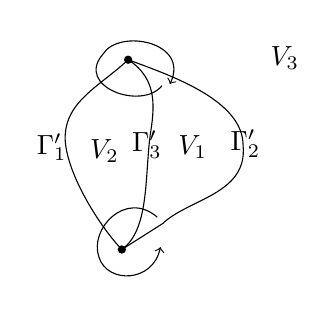
\begin{tikzpicture}[x=1cm,y=1cm]
\draw (1.08,2.56) .. controls (0.72,2.22) and (0.27,2.03) .. (0.28,1.55)
 .. controls (0.30,1.10) and (0.73,0.43) .. (1.00,0.15);
\draw (1.08,2.56) .. controls (1.47,2.31) and (1.41,1.93) .. (1.36,1.60)
 .. controls (1.29,1.07) and (1.35,0.40) .. (1.00,0.15);
\draw (1.08,2.56) .. controls (1.65,2.35) and (2.54,2.04) .. (2.54,1.47)
 .. controls (2.60,0.85) and (1.84,0.79) .. (1.52,0.48) -- (1.00,0.15);
\draw[->] (1.51,2.23) .. controls (1.25,1.91) and (0.40,2.22) .. (0.76,2.63)
 .. controls (0.96,2.96) and (1.87,2.79) .. (1.61,2.25);
\draw[->] (1.45,0.56) .. controls (1.05,0.91) and (0.58,0.41) .. (0.71,0.05)
 .. controls (0.82,-0.29) and (1.40,-0.27) .. (1.49,0.18);
\fill (1.08,2.56) circle (1.5pt); \fill (1.00,0.15) circle (1.5pt);
\node at (0.11,1.45) {$\Gamma'_1$}; \node at (0.78,1.40) {$V_2$};
\node at (1.32,1.48) {$\Gamma'_3$}; \node at (1.90,1.45) {$V_1$};
\node at (2.57,1.49) {$\Gamma'_2$}; \node at (3.07,2.58) {$V_3$};
\end{tikzpicture}}

$\Gamma'_{\unsure{i|\alpha}}\qquad \alpha\in \unsure{I|A}$ ens \unsure{à|:} \unsure{trois él.}
chemin simple joignant les deux \unsure{point|points} de $\unsure{\delta|\partial}=\{x,y\}$

$\Gamma_i=\displaystyle\bigcup_{\underline{\unsure{j|\beta}}\in A-\{i\}}\Gamma'_j$
détermine un ens $B_i$ de \unsure{card.|Card.} 2 (\unsure{l'une|l'un} des 2 régions \unsure{du|de} \deleted{\unsure{pl.}}\inserted{$X$})

\[
 B=\coprod_{i\in I} B_i\qquad
 \text{\deleted{\unsure{:|.} \unsure{quotient|points|graphe} de 3 \unsure{côtés|arêtes}}}
\]

Si $i\in I$ est donné, on lui associe $U_i$ la région de $\Gamma_i$ qui contient $\Gamma'_i-\delta$ \inserted{$=\Gamma_i^{\prime\circ}$}, d'où section de la \unsure{sur. quelle|surj. quelle|sur quelle}
\[
 B\simeq I\times\{0,1\},\qquad V_i
\]

\[
\begin{aligned}
 U_i&=\overset{\circ}{\Gamma}'_i\cup\bigcup_{j\in I\setminus\{i\}}U_j\\
 V_i&=\bigcap_{j\in I\setminus\{\unsure{i|1}\}}V_j
\end{aligned}
\qquad\Bigg/\qquad
\left\{\begin{gathered}
 V_1,V_2,V_3\\ \Gamma_1^\circ,\Gamma_2^\circ,\Gamma_3^\circ\\ \delta
\end{gathered}\right.
\quad
\left\{\begin{aligned}
 U_1&=V_2\cup V_3\cup\Gamma_1^\circ\\
 U_2&=V_3\cup V_1\cup\Gamma_2^\circ\\
 U_3&=V_1\cup V_2\cup\Gamma_3^\circ
\end{aligned}\right.
\]
\[
 U_i,U_j,\ U_k\qquad\Bigg/\qquad
\begin{aligned}
 V_3&=U_1\cap U_2\\
 V_2&=U_3\cap U_1\\
 V_1&=U_1\cap U_2
\end{aligned}
\quad
\left\{\begin{aligned}
 \Gamma_1&=\Gamma_2^\circ\cup\Gamma_3^\circ\cup\delta\\
 \Gamma_2&=\Gamma_3^\circ\cup\Gamma_{\unsure{1|2}}^\circ\cup\delta\\
 \Gamma_3&=\Gamma_1^\circ\cup\Gamma_2^\circ\cup\delta
\end{aligned}\right.
\]

$C$ courbe simple fermée dans surface connexe \deleted{$\unsure{X|K}$}$E$. Conditions équ.

a) card $\pi_0(\deleted{X}E-C)=2$ \quad (\uline{NB} on a tjrs card $\pi_{\unsure{0|{}}}(E-C)\le 2$)

b) $\exists$ ouvert $U\subset\unsure{C|E}$ tel que $\dot U(\overset{\text{dfn}}{=}\overline U-U)=C$ et que \deleted{\unsure{vide|de}}
$\overline U\ne E$ i.e. $V=\overline U-U\ne\emptyset$ i.e. $U\ne E\setminus C$.
% slanted
\margin{($U$ est alors une comp. connexe de $X-C$)}

c) (étant donné un disque $D_x$ assez petit \unsure{centré|\deleted{centré}} en $x\in C$\unsure{\}|)}, et un point $x'$ et un point $x''$ $\in D_x-D_x\cap C$ de part et d'autre de $D_x\cap C$ ....)
$x$ et $y$ n'appart\unsure{iennent|\deleted{iennent|ent}} \unsure{pas|ps.} à la $=$ \unsure{composante} connexe de $X-C$, i.e. $\nexists$ arc \unsure{ds|dans} $X-C$ joignant $x$ \unsure{:|à} $y$.
(\unsure{Car|La} $\{x,y\}\longrightarrow\pi_0(X-C)$ est surjectif ...)
\scanpage{19}
% archive sheet number: 18
\uline{Proposition}\qquad Soient $\Gamma,\Gamma'$ deux \unsure{J.polygônes|J-polygônes} \unsure{sur|du} plan $E$, tels que $\Gamma\cap\Gamma'=I$ soit un arc polygonal non réduit \unsure{à|:} un point. Alors on est dans l'un des deux cas suivants (s'excluant mutuellement)

\[
\begin{aligned}
 &\mathrm{a)}\quad \Gamma-I\subset\mathrm{Ext}(\Gamma'),\quad
 \Gamma'-I\subset\mathrm{Ext}(\Gamma)\\
 &(\Longleftrightarrow\quad \mathrm{Int}\,\Gamma'\subset\mathrm{Ext}\,\Gamma,\quad
 \mathrm{Int}\,\Gamma\subset\mathrm{Ext}\,\Gamma')
\end{aligned}
\]
\[
\begin{aligned}
 &\mathrm{b)}\quad\Gamma-I\subset\mathrm{Ext}\,\Gamma',\quad
 \Gamma'-I\subset\mathrm{Int}\,\Gamma\quad \text{(ou inversement)}\\
 &(\Longleftrightarrow\quad \mathrm{Int}\,\Gamma'\subset\mathrm{Int}\,\Gamma,\quad
 \mathrm{Ext}(\Gamma)\subset\mathrm{Ext}\,\Gamma'\quad \text{(ou \unsure{inv.})})
\end{aligned}
\]

\deleted{\unsure{a)|$\alpha$)} Dans le cas a),}
Soit $\Gamma''=(\Gamma\cup\Gamma')-(I\unsure{\setminus|-}\partial I)
=\overline{\Gamma-I}\cup\overline{\Gamma'-I}$, qui est un polygône.
C'est un J-polygône, et on a :

\[
\begin{aligned}
 \text{\uline{Cas a)}}\quad \mathrm{Int}\,\Gamma''&=\mathrm{Int}\,\Gamma\cup\mathrm{Int}\,\Gamma'\cup(I-\partial I)\\
 \mathrm{Ext}\,\Gamma''&=\mathrm{Ext}\,\Gamma\cap\mathrm{Ext}\,\Gamma'
\end{aligned}
\]
% The circled item in the second line is carried up to the gap after en.
\noindent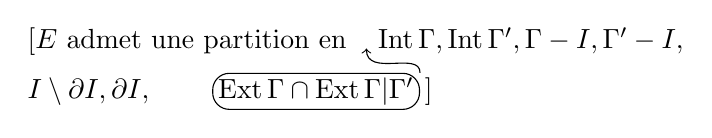
\begin{tikzpicture}[baseline=(lead.base)]
\node[anchor=base west,inner sep=0pt] (lead) at (0,0) {[$E$ admet une partition en};
\node[anchor=base west,inner xsep=2pt,inner ysep=1.5pt,draw,rounded corners=6pt]
 (moved) at (2.35cm,-1.8em)
 {\inserted{$\mathrm{Ext}\,\Gamma\cap\mathrm{Ext}\,\unsure{\Gamma|\Gamma'}$}};
\node[anchor=base west,inner sep=0pt] at ([xshift=1.1em]lead.base east)
 {$\mathrm{Int}\,\Gamma,\mathrm{Int}\,\Gamma',\Gamma-I,\Gamma'-I,$};
\node[anchor=base west,inner sep=0pt] at (0,-1.8em) {$I\setminus\partial I,\partial I,$};
\node[anchor=base west,inner sep=0pt] at ([xshift=.15em]moved.base east) {]};
\draw[->] (moved.north east) .. controls +(0,.8em) and +(0,-1.05em)
 .. ([xshift=.7em]lead.base east);
\end{tikzpicture}

\[
\begin{aligned}
 \text{\uline{Cas b)}}\quad \mathrm{Int}\,\Gamma''&=
 \mbox{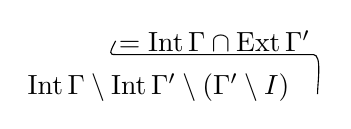
\begin{tikzpicture}[baseline=(mainterm.base)]
 \node[anchor=base west,inner sep=0pt] (mainterm) at (0,0)
 {$\mathrm{Int}\,\Gamma\setminus\mathrm{Int}\,\Gamma'\setminus(\Gamma'\setminus I)$};
 \node[anchor=base east,inner sep=1pt] (addition)
 at ([xshift=.85em,yshift=1.55em]mainterm.base east)
 {$\inserted{=\mathrm{Int}\,\Gamma\cap\mathrm{Ext}\,\Gamma'}$};
 \draw (addition.west) .. controls +(-.23em,-.45em) and +(-.24em,0) .. (addition.south west)
 -- (addition.south east) .. controls +(.32em,0) and +(0,.42em)
 .. ([xshift=1em]mainterm.base east);
 \end{tikzpicture}}\\
 \mathrm{Ext}\,\Gamma''&=\mathrm{Ext}\,\Gamma\cup\mathrm{Int}\,\Gamma'\cup(I\setminus\partial I)
\end{aligned}
\]
[$E$ admet une partition en \inserted{$\mathrm{Ext}\,\Gamma$}
$\mathrm{Int}\,\Gamma\cap\mathrm{Ext}\,\Gamma',\mathrm{Int}\,\Gamma',$
\deleted{$\unsure{\mathrm{Ext}\,\Gamma|\mathrm{Int}\,\Gamma}$}
$\Gamma-I,\Gamma'-I,I-\partial I,\partial I$]
